\begin{appendices}

\section{Abbreviations}

Here we report a list of common abbreviation:

\begin{itemize}
\item \textbf{EOS}: equation of state.
\item \textbf{PV}; parity violating experiment.
\item \textbf{BNSSA}: beam normal single spin asymmetry.
\item \textbf{ENMO}: energy monitor.
\item \textbf{PIMO}: current monitor.
\item \textbf{VFC}: voltage to frequency converter.
\item \textbf{PMT}: photomultiplier tube.
\item \textbf{RTM}: race track microtron.
\item \textbf{XYMO}: position monitor.
\end{itemize} 

\section{Transverse asymmetry}

\section{Data Tree}

In this section we discuss briefly the functions implemented to fill the data tree, from the monitor raw values. In the majority of the \transv experiments, the position of the beam respect to the transverse plane is measured in three different position (see next figure). The three monitors are named XY21, XY25, XY26. During this beam time, only two monitors were available, XY25 and XY21. 

\begin{figure}[hbtp]
\centering
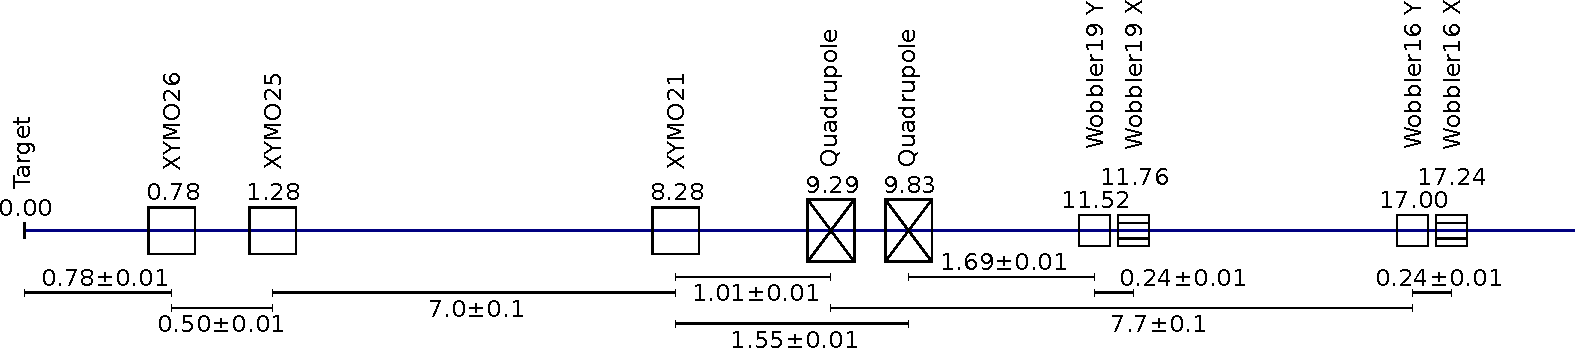
\includegraphics[width = 0.75\textwidth]{figures/XYMOCalibBeamLine.pdf}
\caption{Scheme of the beam line, the target is on the left side of the picture.}
\end{figure}

Other monitors that were used are I21 and E18, the current monitor and energy monitor, respectively. In the figure above, the current monitor correspond to XY21, we have already explained that a resonant cavity can be used to measure both the position and the intensity of the beam, thank to the different modes that are excited by the traveling particles. The E18 monitor, named also ENMO, is not shown in this picture, because it is placed in the racetrack RTM3 (see figure \ref{fig:Accelerator}). 
The raw values from these monitors are collected and stored in binary files, and are made by integers numbers, the digital output of the VFCs. Before the calculation of the important parameters, it is necessary to retrieve to obtain from the raw counts the output voltage of the various monitors. The converting formula is given in equation \ref{eq:Vfc}. The voltage values $V$ are needed to compute the physical quantities, with a simple conversion formula:

\begin{equation}
\dfrac{V \cdot scale - offset}{I}
\end{equation}

In the above formula we divide by the beam current $I$, because the output signal of position and energy the monitors are proportional to the intensity of the beam, and need to be normalized. For the current monitor, the signal is directly proportional to the current, so the denominator is omitted.
The important quantities that are computed by the analysis program are: $X$, $Y$, position of the beam on the target, $\theta_{x}$ and $\theta_{y}$ scattering angles, current $I$ and energy $E$. 
We now briefly present the function implemented to process the raw data and retrieve these quantities.
The position $X$ and $Y$ are computed as explained in section \ref{}. In brevity, assuming that the beam is moving in a straight line, the  beam trajectory is described by:

\begin{align*}
y &= m_{y} \cdot z + q_{y} \\
x &= m_{x} \cdot z + q_{x}
\end{align*}

The values that we are looking for are $q_{x}$ and $q_{y}$, x and y intercept. 
Imposing in the above equations the passage through the points ($Z_{25}$;$X_{25}$) and ($Z_{21}$;$X_{21}$), the intercepts of the equation are given by:

\begin{equation}
q_{x} = \dfrac{Z_{25} \cdot X_{21} - Z_{21} \cdot X_{25}}{Z_{25} - Z_{21}}
\end{equation} 

The scattering angles $\theta_{x}$ and $\theta_{y}$ are instead related to the slope $m$, knowing that $tan(\theta) = m$. The angles are given by the formula:

\begin{equation}
\theta_{x} = \dfrac{X_{25} - X_{21}}{Z_{25} - Z_{21}}
\end{equation}

With these values, the analysis program compute the correlated differences for the angle and position parameter, that are the independent variables for the linear fit.


\end{appendices}